\documentclass[12pt]{article}

\usepackage[affil-it]{authblk}
\usepackage[shortlabels]{enumitem}
\usepackage[utf8]{inputenc}
\usepackage{algorithm, algorithmicx, algpseudocode}
\usepackage{amsfonts, amsthm, amsmath, amssymb}
\usepackage{color}
\usepackage{cancel, textcomp}
\usepackage{enumerate}
\usepackage[mathscr]{euscript}
\usepackage{fancyhdr, fancyvrb}
\usepackage{fullpage}
\usepackage[left=0.5in,right=0.5in,headsep=0.5in,headheight=0.5in]{geometry}
\usepackage{graphicx}
\usepackage{hyperref}
\usepackage{latexsym}
\usepackage{mathtools}
\usepackage{minted}
\usepackage{times}
\usepackage{xcolor}
\usepackage{physics}
\usepackage{tikz-cd}
\usepackage[warnunknown, fasterrors, mathletters]{ucs}
\usepackage[nointegrals]{wasysym}

\newcommand{\hw}[2]{
    \noindent
    \begin{center}
        \framebox{
            \vbox{
                \hbox to 7in { {\bf MATH 470: Communications and Cryptography } \hfill  }
                \vspace{2mm}
                \hbox to 7in { {\Large \hfill Homework #1\hfill} }
                \vspace{2mm}
                \hbox to 7in { {\it Due date: #2 \hfill Name: Huy Lai } }
            }
        }
    \end{center}
    \vspace*{4mm}
}

\newcounter{prob}
\setcounter{prob}{0}
\newcounter{subprob}
\setcounter{subprob}{0}

\newcommand{\problem}{\setcounter{subprob}{0}\stepcounter{prob}{\noindent\textbf{Problem \theprob.}}\ }
\newcommand{\subproblem}{\stepcounter{subprob}{\noindent\textbf{Subproblem \thesubprob.}}\ }
\newcommand{\solution}{\noindent\textbf{Solution:}\newline}

\newcommand{\babc}{\begin{enumerate}[a)]}
\newcommand{\eabc}{\end{enumerate}}

\everymath{\displaystyle}

\setlength{\parskip}{.1in}
\setlength{\headheight}{15pt}
\setlength{\topmargin}{0pt}

\fancyhf{}
\pagestyle{fancy}
\lhead{MATH 470: Communications and Cryptography}
\rhead{Texas A\&M University}
\cfoot{\thepage}


\begin{document}
\hw{1}{30 August 2023}
\thispagestyle{empty}
\problem Decode the following Caesar cipher:
\begin{center}
EREKK MIHSI WRSXP MIGLI EXSVW XIEPS VXSPI VEXIX LSWIA LSHS
\end{center}

\solution
A shift of the encoded message by $4\leftarrow$ or by $22\rightarrow$ would decode the message\\
ANAGG IEDOE SNOTL IECHE ATORS TEALO RTOLE RATET HOSEW HODO

\noindent
This message can be further parsed into the following:\\
An Aggie does not lie cheat or steal or tolerate those who do

\problem Encrypt the plaintext message using the subsitution encryption table
\begin{table}[!ht]
    \centering
    \begin{tabular}{|c|c|c|c|c|c|c|c|c|c|c|c|c|c|c|c|c|c|c|c|c|c|c|c|c|c| }
        \hline
        A & B & C & D & E & F & G & H & I & J & K & L & M & N & O & P & Q & R & S & T & U & V & W & X & Y & Z \\
        \hline
        S & C & J & A & X & U & F & B & Q & K & T & P & R & W & E & Z & H & V & L & I & G & Y & D & N & M & O \\
        \hline
    \end{tabular}
    \caption{Simple substitution encryption table}
\end{table}

\noindent
Plain Text:
\begin{center}
The gold is hidden in the garden
\end{center}

\solution
``IBXFE PAQLB QAAXW QWIBX FSVAX W"

\newpage
\problem Let $a,b,c\in\mathbb{Z}$. Use the definition of divisibility to directly prove that if $a\mid b$ and $b\mid a$, then $a=\pm b$.

\solution 
Prove that if $a\mid b$ and $b\mid a$, then $a=\pm b$
\begin{proof}
By definition $\exists x,y\in\mathbb{Z}$ such that $a=bx$ and $b=ay$\\
$a = bx \Rightarrow a = ayx$\\
Dividing both sides by $a$ results in:\\
$1 = yx$

\noindent
Since both $x$ and $y$ are integers and their product is 1, $x=y=\pm 1$\\
Using this result in the equation for $a$ gives:\\
$a=\pm b$
\end{proof}

\problem Use the Euclidean algorithm to compute the greatest common divisor of 291 and 252.

\solution
$\gcd(291,252)$
\begin{flalign*}
292 &= 1*252+40 &\\
252 &= 6*40+12 &\\
40 &= 3*12+4 &\\
12 &= 3*4+0 &
\end{flalign*}
$\gcd(291,252)=3$

\newpage
\problem Let $a$ and $b$ be positive integers.

\subproblem Suppose that there are integers $u$ and $v$ satisfying $au+bv=1$. Prove that $\gcd(a,b)=1$.

\solution Prove that $\gcd(a,b)=1$.
\begin{proof}
Let $g=\gcd(a,b)$. Then $\exists x,y\in\mathbb{Z}$ such that $a=gx\land b=gy$\\
Substituting this into the given equation $au+bv=1$ results in:
\[
1=au+bv=gxu+gyv=g(xu+yv)
\]

\noindent
$u,v,x,y\in\mathbb{Z}\rightarrow(xu+yv)\in\mathbb{Z}$\\
As a result of the previous statement:\\
$g\mid 1$\\
This requires that $g=1$.
\end{proof}

\newpage
\subproblem Suppose that there are integers $u$ and $v$ satisfying $au+bv=6$. Is it necessarily true that $\gcd(a,b)=6$? If not, give a specific counterexample, and describe in general all of the possible values of $\gcd(a,b)$?

\solution
$au+bv=6$ does not imply that $\gcd(a,b)=6$.\\
Counterexample: $a=3,b=2$
\[a\cdot(6)+b\cdot(-6)=6\]
but $\gcd(a,b)=1$

\noindent
In general, if $au+by=c$ has a solution, then $\gcd(a,b)|c$.\\
Let $g=\gcd(a,b)$. Divide $c$ by $g$ with remainder $r$ such that
\[c=gq+r \textrm{ with } 0\leq r< g\]
We know that we can find a solution to $g=ax+by$, so we get
\[au+bv=c=gq+r=(ax+by)q+r\]
Rearranging this statement results in:
\[a(u-xq)+b(v-yq)=r\]

\noindent
The left hand side is divisible by $g$ since $\gcd(a,b)=g$. Therefore, $g\mid r$. But the only $r$ that can satisfy both $0\leq r < g$ and $g\mid r$ is $r=0$. This results in $c=gq$. This implies that $\gcd(a,b)|c$.

\noindent
It is not hard to see that each divisor of 6 can be obtained as the gcd of two integers.\\
For example $1(1)+5(1)=2(1)+4(1)=3(1)+3(1)=6(1)+0(1)=6$\\
The corresponding $\gcd(a,b)$ are $1,2,3,6$ respectively.

\newpage
\problem Find the gcd of the following two numbers:
\begin{flalign*}
a &= 1234567890123456789012345678901234567890123456789012345678901234567890123456789 \\
b &= 234567890123456789012345678901234567890123456789012345678901234567890123456789
\end{flalign*}

\solution
\begin{minted}{python}
def gcd(a: int, b: int):
    if a == 0:
        return b
    if b == 0:
        return a
    return gcd(b, a % b)


def main():
    a = 1234567890123456789012345678901234567890123456789012345678901234567890123456789
    b = 234567890123456789012345678901234567890123456789012345678901234567890123456789

    print("gcd(a,b) =", gcd(a, b))


if __name__ == "__main__":
    main()
\end{minted}

\begin{figure}[ht!]
    \centering
    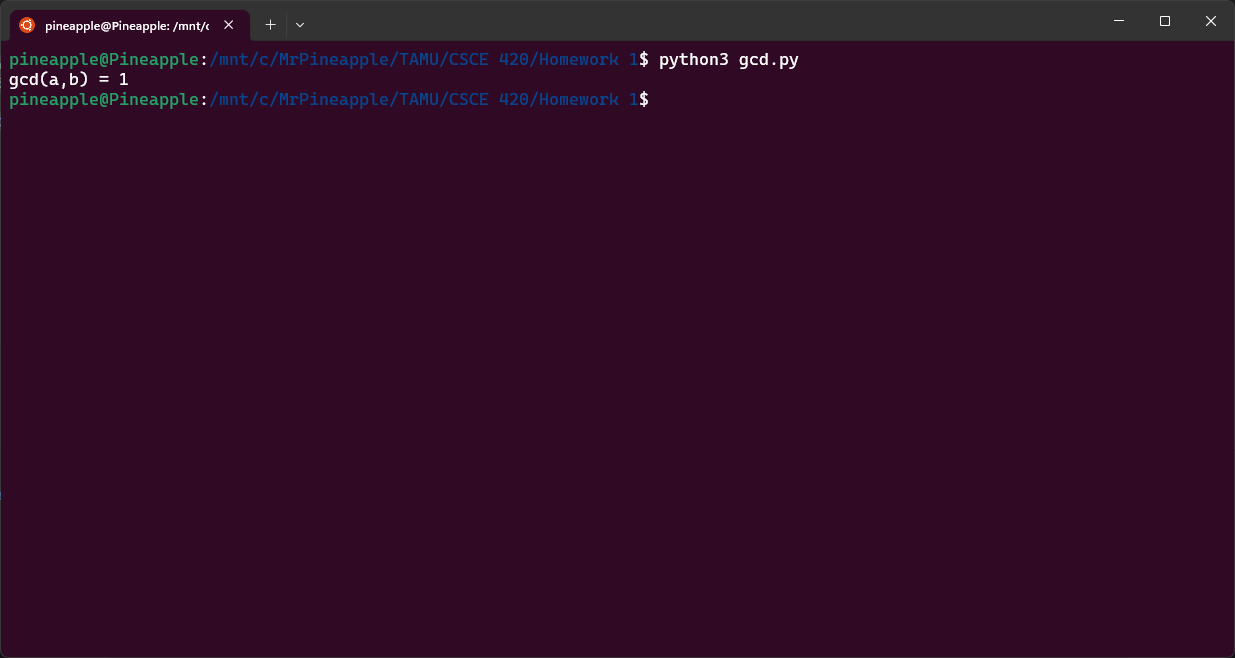
\includegraphics[width=\textwidth]{Problem 6.png}
    \caption{Output of the Code}
\end{figure}

\end{document}
